% To je predloga za poročila o domačih nalogah pri predmetih, katerih
% nosilec je Blaž Zupan. Seveda lahko tudi dodaš kakšen nov, zanimiv
% in uporaben element, ki ga v tej predlogi (še) ni. Več o LaTeX-u izveš na
% spletu, na primer na http://tobi.oetiker.ch/lshort/lshort.pdf.
%
% To predlogo lahko spremeniš v PDF dokument s pomočjo programa
% pdflatex, ki je del standardne instalacije LaTeX programov.

\documentclass[a4paper,11pt]{article}
\usepackage{a4wide}
\usepackage{fullpage}
\usepackage[utf8x]{inputenc}
\usepackage[slovene]{babel}
\usepackage{caption}
\usepackage{subcaption}
\selectlanguage{slovene}
\usepackage[toc,page]{appendix}
\usepackage[pdftex]{graphicx} % za slike
\usepackage{setspace}
\usepackage{color}
\definecolor{light-gray}{gray}{0.95}
\usepackage{listings} % za vključevanje kode
\usepackage{hyperref}
\usepackage{float}
\usepackage{varwidth}
\renewcommand{\baselinestretch}{1.2} % za boljšo berljivost večji razmak

\newcommand{\rulesep}{\unskip\ \vrule\ }

\lstset{ % nastavitve za izpis kode, sem lahko tudi kaj dodaš/spremeniš
language=Python,
basicstyle=\footnotesize,
basicstyle=\ttfamily\footnotesize\setstretch{1},
backgroundcolor=\color{light-gray},
}

\title{Inteligentni sistemi, 2. seminarska naloga}
\author{Matic Bernik in Robert Tovornik}
\date{17. januar 2017}

\begin{document}

\maketitle

\section{Uvod}

Glavna tema druge seminarske naloge je tekstovno rudarjenje ter tekstovna klasifikacija. Naloga je bila sestavljena 
iz več delov. V prvem delu sva izbrala klasifikacijski kriterji, torej lastnost, ki jo bova iz podatkov napovedovala. Izbrala sva 
napovedovanje avtorja teksta ter spol avtorja. Nato je sledilo dejansko rudarjenje (zbiranje knjig) ter izgradnja korpusa. 
Sledillo je procesiranje ter obdelava zbranih dokumentov ter tvorjenje znacilk (atributov). Za konec je preostala še klasifikacija 
dokumentov. Uporabila sva več metod: SVM, naključne gozdove, naivnega Bayesa ter večinski klasfikator.

\section{Podatki}

Podatki za nalogo, ki so hrajeni v korpusu, so tekstovne knjige zbrane s spletne strani projekta Gutenberg.
 Vsa dela so bila zbrana v skladu s pravili (uporaba knjižnice R - gutenbergr), preko zrcala. V korpusu so zbrana dela 26 različnih avtorjev, 
v angleškem jeziku. Hranjena so v direktoriju "books". Ta se nato deli na poddirektorije z imeni avtorjev, ter slednji na dva nova,
 "txt" ki vsebuje knjige v formatu .txt, ter "header", ki vsebuje datoteke z metapodatki o soimenski knjigi, dostopni s strani gutenberg. 
V nadalji obdelavi, sva dela razčlenila na "članke", po principu delitve vsakega dela na 20 člankov, kjer vsak vsebuje minimalno 500 besed. 
Posledično, so nekatera dela, ki zaradi pomanjkanja števila besed niso ustrezala pogojem, izpadla. Na koncu nama je ostalo cca. 7200 člankov.

Glavni problem, na katerega je pri deljenju na članke potrebno biti pozoren, je dejstvo da ima vsaka knjiga na začetku zapisane meta 
podatke in informacije o samem delu, morda tudi avtorju. Problem sva rešila tako, da pri vsakem delu preskočiva nekaj začetnih odstavkov.

\section{Predprocesiranje podatkov}

Da poenostavimo procesiranje, ustvarjanje atributov, zmanjšamo število kombinacij, ter da lažje iščemo povezave 
med besedili, je tekstovne datoteke najprej potrebno predobdelati. Tu pridejo na vrsto klasični postopki, kot so transformacija 
teksta v male črke, korenizacija, razbijanje na tokene, besede,.. Pri navedenih postopkih sva si pomagala z python knjižnjico nltk.

\section{Izbor ter obdelava klasifikacijskih atributov}

Ker sva se odločila za napovedovanje avtorjev, teksta, sva morala poiskati atribute, ki nekako definirajo in hkrati ločijo, 
torej dobro diskiminirajo med lastnostmi posamezniih avtorjev. Zato sva kot osnovo izbrala atribute frekvenc pojavitve 
nabora "posebnih znakov", to so vejice, pike, narekovaji, dvopicja,.. Kasneje se je izakalo kot zelo učinkovito. Nato 
sva sestavljala bolj zapletene atribute, ki so zajemala neko povezavo - razmerje znotraj besedila. Npr.: razmerje med
 številom stavkov ter besed v besedilu, povprečno dolžino stavka,.. Za konec sva sestavila še nabor najpogosteje uporabljenih besed, 
ozrioma število pojavitev le-teh. Tudi ti atributi so se izkazali kot uspešni. 

\begin{figure}[H]
\begin{center}
\centering
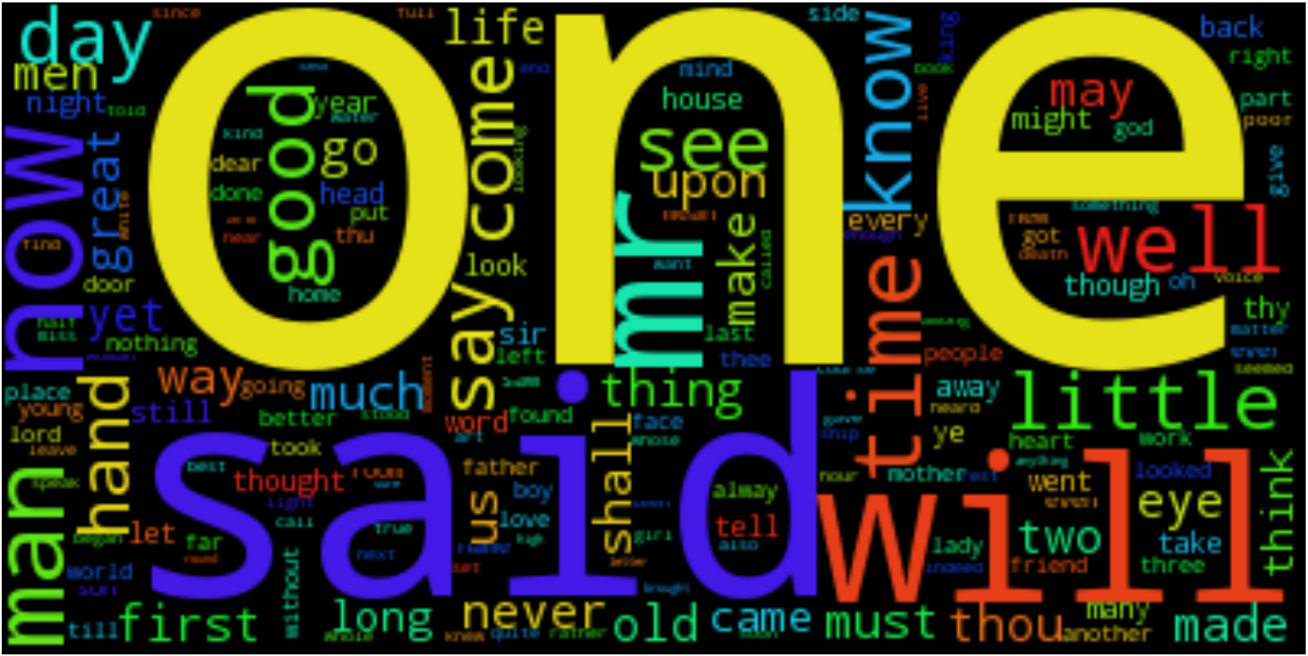
\includegraphics[scale=0.4]{worldCloudPy-skaliran-nabor-wo-202d.PNG}
\caption{Skaliran nabor najpogostejših besed v korpusu.}
\label{slika1}
\end{center}
\end{figure}


Hitro sva ugotovila, da ker so izbrane knjige različnih velikosti, deliva pa vse po enakem postopku prihaja do velikih razlik pri izračunih.
Zato je bilo potrebno vse frekvence tudi normalizirati. Nekatere z dolžino besedila, druge s številom vseh besed, stavkov,..

To je pripeljalo do dodatnih izboljšav v napovedovanju. Približno 4 odstotke.

\section{Klasifikacija ter klasifikacijska točnost}

Pred pričetkom učenja klasifikacijskih modelov, je bilo potrebno zgraditi dodatno datoteko "dataset.tab", kjer vsaka 
vrstica predstavlja posamezen članek (delo) ter iz podatkov izpeljane pripadajoče vrednosti značilk.

Pred začetkom klasifikacije, sva uporabila oceno nad atributi (information gain, relieff), da sva potrdila ustreznost izbranih attributov.\\

\begin{figure}[H]
\centering
\begin{subfigure}{0.48\textwidth}
  \centering
  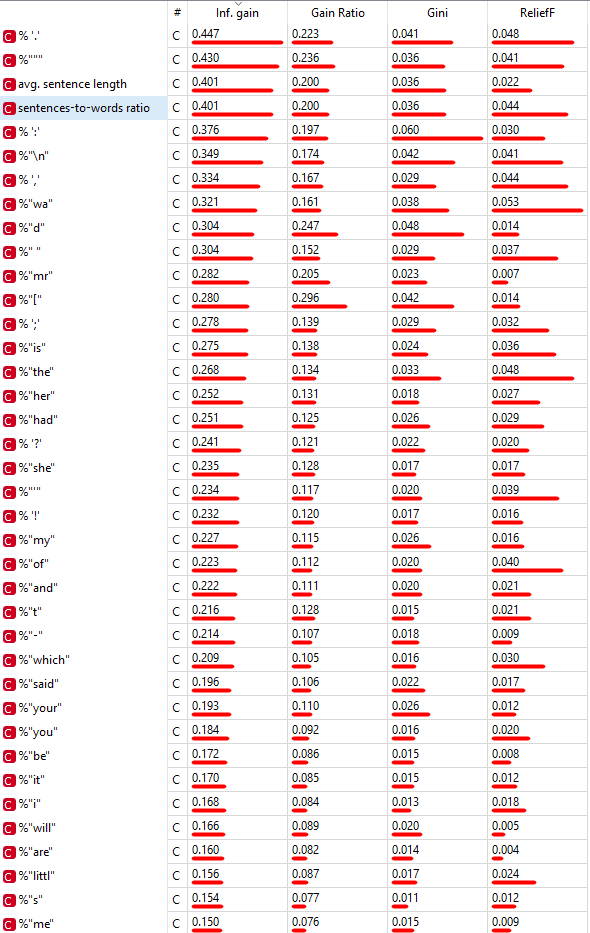
\includegraphics[scale=0.5]{authors_small_infG.png}
  \caption{Za avtorja}
  \label{slika2}
\end{subfigure}%
\rulesep
\begin{subfigure}{0.48\textwidth}
  \centering
  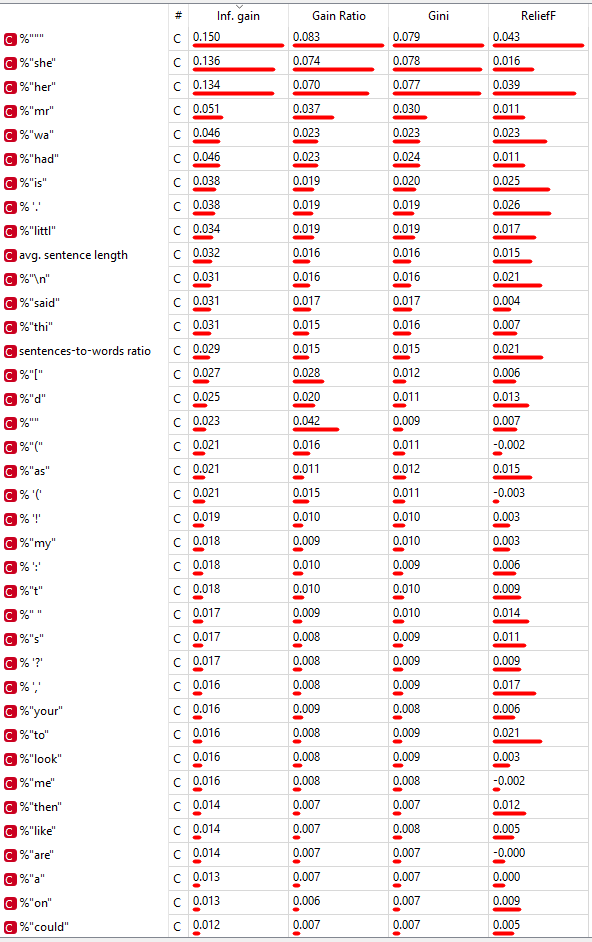
\includegraphics[scale=0.5]{gender_small_infG.png}
  \caption{Za spol avtorja}
  \label{slika3}
\end{subfigure}
\caption{Primernost klasifikacijskih atributov}
\label{fig:test}
\end{figure}

Tukaj lahko opazimo zanimivost pri napovedovanju spola avtorja, kjer je nenadoma prišlo do večjega preskoka v informacijskem 
pridobitku. Velik del namreč pridobijo besede, ki definirajo spol ('her', 'she'),.

Za učne modele sva izbrala več klasifikatorjev: večinski klasifikator, naivni Bayesov, k najbližjih sosedov, SVM ter naključne gozdove.
Kot predvideno po teoriji, se je tudi tukaj izkazalo, da so najprimernješi prav, NB, SVM, ter RF.

Rezultati so sledeči.\\

\begin{table}[ht]
  \begin{varwidth}[b]{0.7\linewidth}
    \centering
    \begin{tabular}{ l | l  l  l  l  l }
    \hline
    Method & AUC & CA & F1 & Precision & Recall \\ \hline \hline
    SVM & 0.914 & 0.843 & 0.835 & 0.841 & 0.843 \\ \hline
    Naive Bayes & 0.843 & 0.704 & 0.704 & 0.727 & 0.704 \\ \hline
    Random Forest & 0.818 & 0.673 & 0.652 & 0.662 & 0.673 \\ \hline
    kNN & 0.564 & 0.197 & 0.182 & 0.185 & 0.197 \\ \hline
    \hline
    Majority & 0.500 & 0.132 & 0.031 & 0.017 & 0.132 \\ \hline \hline
    \end{tabular}
    \caption{Klasifikacijska točnost pri napovedovanju avtorja}
    \label{table:tocnost}
  \end{varwidth}%
  \hfill
  \begin{minipage}[b]{0.3\linewidth}
    \centering
    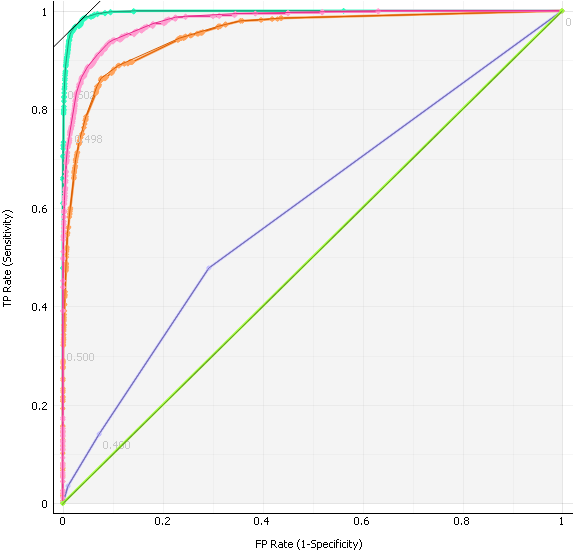
\includegraphics[scale=0.2]{authors_ROC.png}
    \captionof{figure}{ROC krivulja}
    \label{slika4}
  \end{minipage}
\end{table}

Pri napovedovanju spola, pa se je točnost napovedih metod močno spremenila. Izstopali so naključni gozdovi, 
kot izredno dober klasifikator, medtem ko je prej najboljši SVM močno padel.

\begin{table}[ht]
  \begin{varwidth}[b]{0.7\linewidth}
    \centering
    \begin{tabular}{ l | l  l  l  l  l }
    \hline
    Method & AUC & CA & F1 & Precision & Recall \\ \hline \hline
    Random Forest & 0.810 & 0.866 & 0.909 & 0.862 & 0.866 \\ \hline
    Naive Bayes & 0.783 & 0.783 & 0.838 & 0.813 & 0.783 \\ \hline \hline
    Majority & 0.500 & 0.720 & 0.837 & 0.518 & 0.720 \\ \hline \hline
    kNN & 0.541 & 0.671 & 0.785 & 0.636 & 0.671 \\ \hline 
    SVM & 0.614 & 0.588 & 0.659 & 0.689 & 0.588 \\ \hline
    \end{tabular}
    \caption{Klasifikacijska točnost pri napovedovanju spola avtorja}
    \label{table:tocnost}
  \end{varwidth}%
  \hfill
  \begin{minipage}[b]{0.3\linewidth}
    \centering
    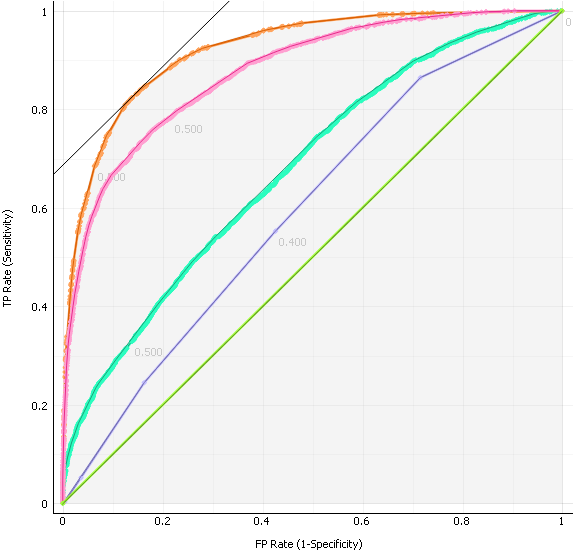
\includegraphics[scale=0.2]{gender_ROC.png}
    \captionof{figure}{ROC krivulja}
    \label{slika5}
  \end{minipage}
\end{table}

Pa še nekaj zanimivih vizualizacij. Confusion matrix, scatter plots.


\begin{figure}[H]
\begin{center}
\centering
  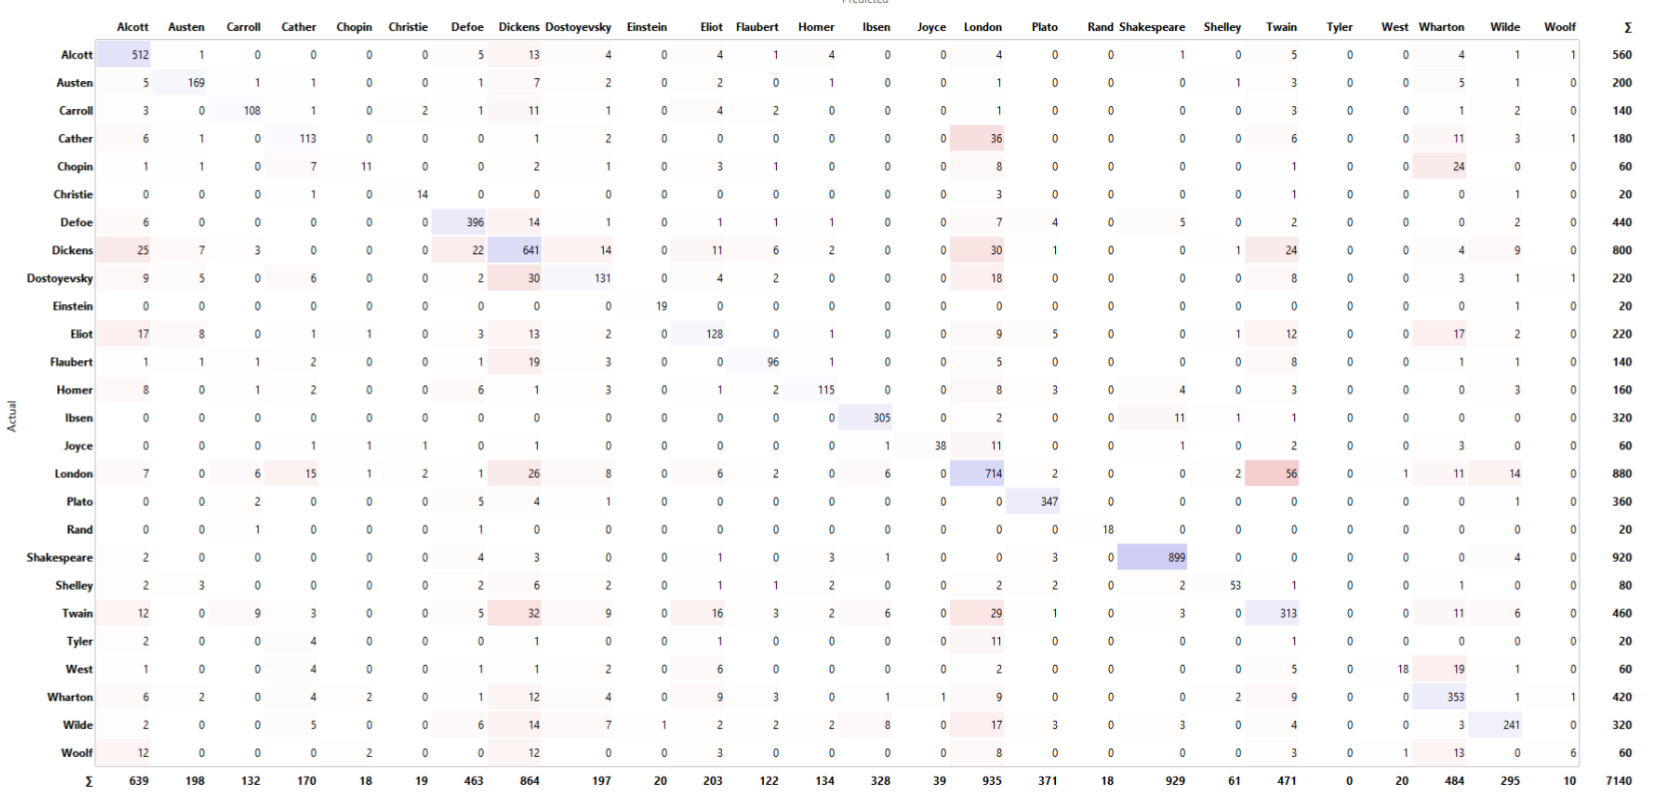
\includegraphics[scale=0.4]{authors_conf_matrix_tight.png}
  \caption{Confusion matrix za avtorja}
  \label{slika6}
\end{center}
\end{figure}

\begin{figure}[H]
\begin{center}
\centering
  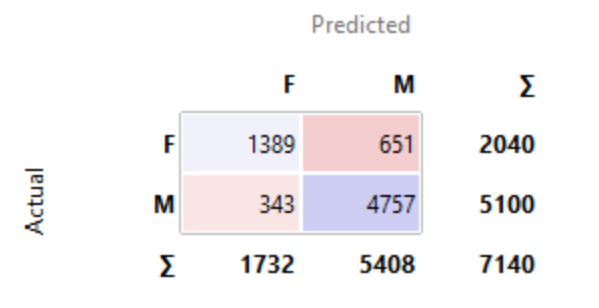
\includegraphics[scale=0.4]{gender_conf_matrix_tight.png}
  \caption{Confusion matrix za spol}
  \label{slika7}
\end{center}
\end{figure}

V konfuzni matriki napovedi avtorja, lahko kot zanimivost opazimo povezavo med največ zgrešenimi napovedmi prav 
med dvema avtorjema, Mark Twain ter Jack London. Če se malce poglobimo, pridemo do podatka, da sta oba avtorja 
ustvarjala v istem obdobju (razlika 10ih let), oba sta pisala pustolovske romane, oba sta pisala v 2. osebi,.. Torej lahko rečemo,
 da obstaja velika podobnost v slogu pisanja.

\section{Zanimivi atributi}

Med prej naštetimi se je nekaj atributov izkazalo kot takih, ki izjemno dobro določajo specifike avtorjev. 
Dva izmed njih sva se odločila izpostaviti.\\

Ker si množice številk težko predstavljamo, sva se odločila da to prikaževa grafično. Tako spodnja slika zelo dobro 
prikazuje razporejanje del k avtorjem, na podlagi ene izmed slovognih specifik (povprečne dolžine stavka). 
Zelo dobro je razvidno, da večina barv spada kamor je treba, izstopa jih le nekaj malo.

\begin{figure}[H]
\begin{center}
  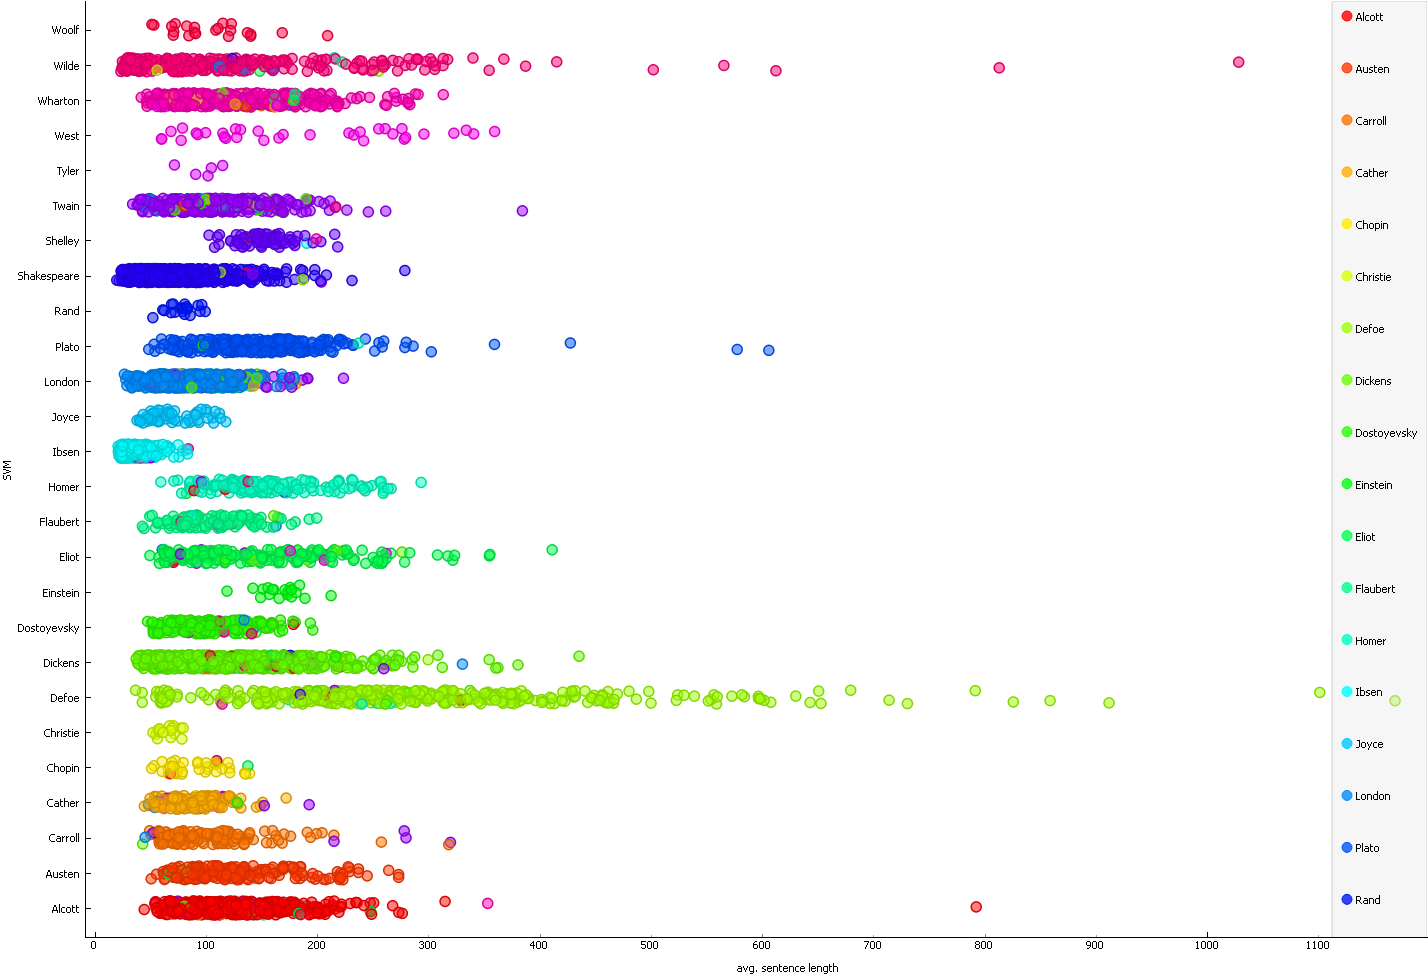
\includegraphics[scale=0.5]{authors_scatter_sent_len_SVM.png}
  \caption{Graf razpršenosti - povprečna dolžina stavka - SVM}
  \label{slika8}
\end{center}
\end{figure}

Drug atribut, ki izjemo izstopa, tokrat pri klasifikaciji spola avtorja, pa je že prej omenjen atribut 'she', torej atribut ki v tekstu 
opredeljuje spol. Če pogledamo graf škatle z brki, lahko vidimo da izjemno natančno opredeljuje vrednosti, saj se večina vrednosti 
nahaja znotraj izjemno majhnega intervala.

\begin{figure}[H]
\begin{center}
\centering
  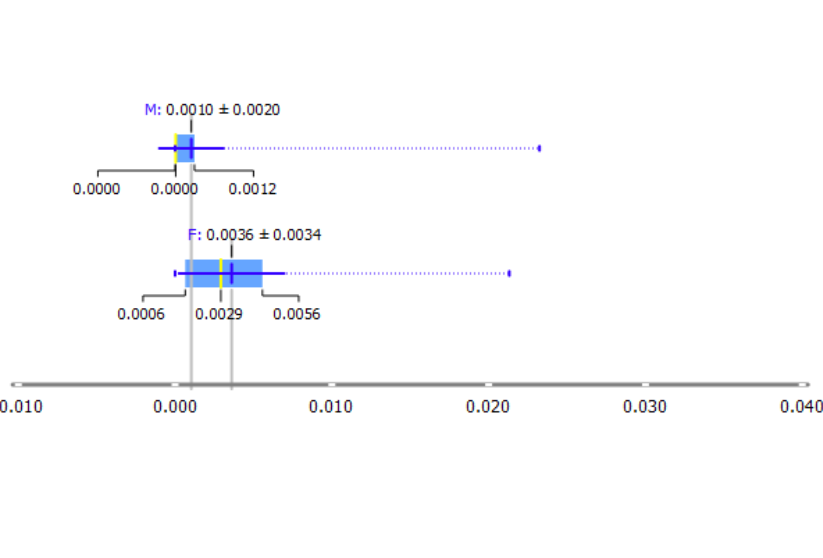
\includegraphics[scale=0.6]{gender_word_she_boxplot_tight.png}
  \caption{Škatla z brki - beseda she}
  \label{slika9}
\end{center}
\end{figure}

\section{Zaključek}

Za konec, bi lahko na vse skupaj pogledali še s prakičnega vidika. Namreč če pogledamo atribute, ki zelo dobro določajo 
avtorje, lahko vidimo nek smisel, ki ga prikazujejo. Na primer.: če opazujemo število uporabljenih ločil, navednic, in pa 
dolžino povprečnih povedi, doližno odstavkov, vidimo da so to pravzaprav lastnosti, ki določajo pisalni slog avtorja.
Po drugi strani če pogledamo najpogostje uporabljene besede v besedilih avtorja, vidimo da to pravzaprav določa razgledanost 
avtorja in njegov besedni zaklad.

\subsection{Stacking}

Kot lahko opazimo, znamo spol napovedovati zelo dobro, bolje kot avtorja samega, saj je nabor dosti večji kot pri spolu, kjer sta (vsaj v večini primerov) 
zgolj dve opciji. Zato lahko pridemo na idejo, da bi napovedni metodi zaporedno združili v upanju izboljšave. Torej najprej napovemo spol, ter ga kot atribut podamo v klasifikator avtorja. Če to naredimo pride do pozitivne spremembe v klasifikacijski točnosti. Nova napovedna točnost avtorja s predhodno najboljšim  klasifikatorjem SVM je 87.8 odstona z podporo AUC 0.933. Pripeljali smo torej do izbolšanja za dobre 3 odstotke. Tehnika torej kaže potencial.


\end{document}